\documentclass[10pt,a4paper]{amsart}
\usepackage[margin=19mm]{geometry}
\usepackage{amsmath,amssymb,mathtools}
\usepackage[scr=rsfs,cal=euler]{mathalfa}
\usepackage{xfrac}
\usepackage[unicode,hidelinks,bookmarks=false]{hyperref}
\newcommand{\ie}{i.e.\ }
\newcommand{\cf}{cf.\ }
\newcommand{\resp}{respectively\ }
\newcommand{\Subsection}{\subsection}
\providecommand{\nobreakdash}{\nobreak\hbox{-}}
\setlength{\emergencystretch}{2em}
\multlinegap0pt
\usepackage{tikz}
\usepackage{amssymb}
\usepackage{xcolor}
\usepackage{enumerate}
\usepackage{bm}
\usepackage{float}
\newtheorem{proposition}{Proposition}
\newtheorem{theorem}{Theorem}
\title{Fourier transform of irregular connections on $\mathbb P^1$ and classification of Argyres--Douglas theories}
\author{Jean Dou\c{c}ot}
\date{Source: arXiv:2603.15942v1 (CC BY 4.0)}
\begin{document}
\maketitle

\noindent\emph{Source and licence.} Fourier transform of irregular connections on $\mathbb P^1$ and classification of Argyres--Douglas theories. Version arXiv:2603.15942v1 (CC BY 4.0), distributed by arXiv under the Creative Commons Attribution 4.0 International licence, http://creativecommons.org/licenses/by/4.0/, as recorded in the arXiv licence metadata for this exact version and shown on the abstract page https://arxiv.org/abs/2603.15942v1. Full licence notice: \texttt{licenses/arxiv-2603.15942-CC-BY-4.0.txt}.\par\smallskip

\noindent\textit{Editorial scope.} Counted unit: the article's theorem fig:structure\_orbit (source0.tex lines 1111--1209). The article's complete original proof of it is delivered with it (source0.tex lines 1211--1227, one \texttt{proof} environment of 17 lines). No mathematics is written, repaired or re-derived: the statement and the proof are the article's own lines, in the article's own notation, and no retained line is substituted or re-flowed.  Retained uncounted as the source-local context the proof needs: lines 995--1014; lines 1495--1512.  Nothing was omitted from any retained span, so the package carries no omission record.  No retained line contains a citation, so the wrapper carries no bibliography and no bibliography entry.  The retained lines contain the article's own diagram code, which the wrapper typesets with the standard tikz packages; no image file is delivered and the package declares no asset dependency.  Editorial formatting only, in addition: an AMS \texttt{amsart} preamble that restates the article's own declarations and macros used by the retained lines, namely the environments \texttt{proposition}, \texttt{theorem} on separate counters, together with the standard packages those lines need.  The retained environments print in this document as Proposition 1, Theorem 1 in order of appearance, whereas the article prints the same items with the numbering of its own full document.  The complete native source of the article as distributed in the arXiv e-print for this exact version is bundled unchanged as \texttt{sources/196509/source0.tex}.
\begin{proposition}
\label{prop:transformation_parameter_elementary_operation_type_I}
Let $\bm\Sigma$ be an irregular curve with boundary data of generalized type I AD-$A$ type, with parameter $\mathcal T=(m,k,[Y^0], [Y^\infty])$. Then, if $O$ is an allowed elementary AD-$A$-operation on $\mathcal T$, the irregular curve with boundary data $O\cdot \bm\Sigma$ is of generalized AD-$A$ type. 

Furthermore, in each case, we have the following explicit expression for the parameter $O\cdot \mathcal T$ of $O\cdot\bm\Sigma$:
\begin{enumerate}
\item If $k>1$, then the irregular curve with boundary data $F\cdot \bm\Sigma$ is  of generalized type I AD-$A$ type, with parameter
\begin{equation}
F\cdot \mathcal T=\left(m,\frac{s}{s-r},[ms-h_1(Y^0),Y^{\infty}], [\tau(Y^{0})]\right).
\end{equation}
\item The irregular curve with boundary data $\widetilde F^+\cdot \bm\Sigma$ is of generalized type I AD-$A$ type, with parameter
\begin{equation}
\widetilde F^+\cdot\mathcal T=\left(m,\frac{s}{s+r},[ms-h_1(Y^\infty),Y^{0}], \tau(Y^{\infty})\right).
\end{equation}
\item If $k<1$, the irregular curve with boundary data $\widetilde F^-\cdot \bm\Sigma$ is of  generalized type I AD-$A$ type, with parameter
\begin{equation}
\widetilde F^-\cdot\mathcal T=\left(m,\frac{s}{r-s},[\tau(Y^{0})], [ms-h_1(Y^0),Y^{\infty}]\right). 
\end{equation}
\end{enumerate}
\end{proposition}

\begin{proposition}
\label{prop:transf_parameter_elementary_transf_twist}
Let $\bm\Sigma$ be an irregular curve with boundary data of generalized  AD-$A$ type, with parameter $\mathcal T=(m,k,\mathcal C_0, \mathcal C_\infty)$, and $\alpha\in \mathbb C^*$. Let $[Y^0_\alpha]$ denote the Young diagram associated to $\alpha$ in the Jordan form of $\mathcal C_0$, and $h:=h_1(Y^0_\alpha)$ the height of its first column. 
\begin{enumerate}
\item If $k\geq 1$, then the irregular curve with boundary data $F_\alpha\cdot \bm\Sigma$ is  of generalized AD-$A$ type, with parameter
\begin{equation}
F_\alpha\cdot \mathcal T:=\left(m,\frac{s}{s-r},\varepsilon_{(ms-h),\alpha}(\mathcal C_{\infty}), \tau_\alpha(\mathcal C_0)\right).
\end{equation}
\item The irregular curve with boundary data $\widetilde F^+_\alpha\cdot \bm\Sigma$ is of generalized  AD-$A$ type, with parameter
\begin{equation}
\widetilde F^+_\alpha\cdot \mathcal T:=\left(m,\frac{s}{s+r},\varepsilon_{(ms-h),\alpha}(\mathcal C_{0}), \tau_\alpha(\mathcal C_\infty)\right) .
\end{equation}
\item If $k<1$, the irregular curve with boundary data $\widetilde F^-_\alpha\cdot \bm\Sigma$ is of  generalized AD-$A$ type, with parameter
\begin{equation}
\widetilde F^-_\alpha\cdot \mathcal T:=\left(m,\frac{s}{r-s},\tau_\alpha(\mathcal C_{0}), \varepsilon_{(ms-h),\alpha}(\mathcal C_\infty)\right).
\end{equation}
\end{enumerate}
\end{proposition}

\begin{theorem}
Let $\mathcal T=(m, k, \mathcal C_0, \mathcal C_\infty)$ be a generalized type I AD-$A$ parameter. Let us write $k=\frac{s}{r}$, with $s, r$ coprime, and assume that $s>1$. Let $r=\kappa s+\rho$ , with $\kappa\in \mathbb Z_{\geq 0}$ and $\rho\in \{1, \dots, s-1\}$ be the euclidean division of $r$ by $s$. 
Then the orbit $\mathcal O(\bm\Sigma)$ has the structure described on Fig. \ref{fig:structure_orbit} below.

\begin{figure}[h]
\centering
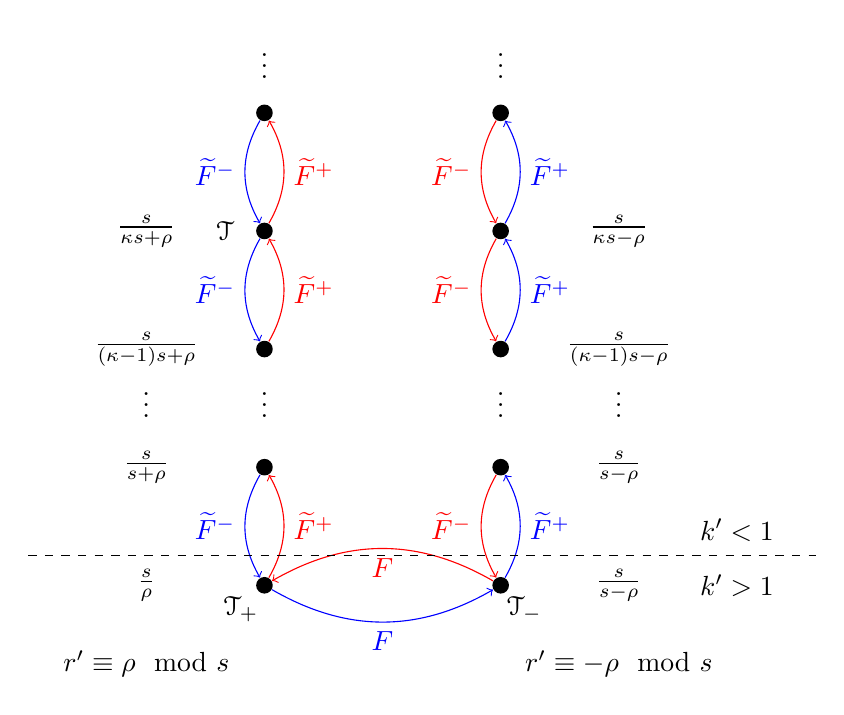
\begin{tikzpicture}
\tikzstyle{vertex}=[circle,fill=black,minimum size=6pt,inner sep=0pt]
\node[vertex] (A0) at (0,0){} ;
\node[vertex] (B0) at (3,0){};  

\draw (-1.5,0) node {$\frac{s}{\rho}$};
\draw (4.5,0) node {$\frac{s}{s-\rho}$};

\draw (-0.3,-0.3) node {$\mathcal T_+$};
\draw (3.3,-0.3) node {$\mathcal T_-$};


\node[vertex] (A1) at (0,1.5)  {};
\node (A2) at (0,2.4)  {$\vdots$};
\node[vertex] (A3) at (0,3) {};
\node[vertex] (A4) at (0,4.5)  {};
\node[vertex] (A5) at (0,6)  {};
\node (A6) at (0,6.7)  {$\vdots$};



\draw (-1.5,1.5) node  {$\frac{s}{s+\rho}$};
\draw  (-1.5,2.4)  node {$\vdots$};
\draw (-1.5,3)  node {$\frac{s}{(\kappa-1) s+\rho}$};
\draw (-1.5,4.5)  node {$\frac{s}{\kappa s+\rho}$};
\draw (-0.5,4.5)  node {$\mathcal T$};


\node[vertex] (B1) at (3,1.5)  {};
\node (B2) at (3,2.4)  {$\vdots$};
\node[vertex] (B3) at (3,3) {};
\node[vertex] (B4) at (3,4.5)  {};
\node[vertex] (B5) at (3,6)  {};
\node (B6) at (3,6.7)  {$\vdots$};

\draw (4.5,1.5) node  {$\frac{s}{s-\rho}$};
\draw  (4.5,2.4)  node {$\vdots$};
\draw (4.5,3)  node {$\frac{s}{(\kappa-1) s-\rho}$};
\draw (4.5,4.5)  node {$\frac{s}{\kappa s-\rho}$};


\draw[red, <-] (A0) to[bend left] node[midway, below]{$F$} (B0);
\draw[blue,->] (A0) to[bend right] node[midway, below]{$F$} (B0);

\draw[red,->] (A0) to[bend right] node[midway, right] {$\widetilde F^+$} (A1);
\draw[blue,->] (A1) to[bend right] node[midway, left] {$\widetilde F^-$} (A0);


\draw[red, ->] (A3) to[bend right] node[midway, right] {$\widetilde F^+$} (A4);
\draw[blue,->] (A4) to[bend right] node[midway, left] {$\widetilde F^-$} (A3);

\draw[red, ->] (A4) to[bend right] node[midway, right] {$\widetilde F^+$} (A5);
\draw[blue,->] (A5) to[bend right] node[midway, left] {$\widetilde F^-$} (A4);


\draw[blue, ->] (B0) to[bend right] node[midway, right] {$\widetilde F^+$} (B1);
\draw[red,->] (B1) to[bend right] node[midway, left] {$\widetilde F^-$} (B0);


\draw[blue,->] (B3) to[bend right] node[midway, right] {$\widetilde F^+$} (B4);
\draw[red, ->] (B4) to[bend right] node[midway, left] {$\widetilde F^-$} (B3);

\draw[blue,->] (B4) to[bend right] node[midway, right] {$\widetilde F^+$} (B5);
\draw[red, ->] (B5) to[bend right] node[midway, left] {$\widetilde F^-$} (B4);

\draw (-1.5,-1) node {$r'\equiv \rho \mod s$};
\draw (4.5,-1) node {$r'\equiv -\rho \mod s$};
\draw[dashed] (-3, 0.38) -- (7,0.38);
\draw (6, 0) node {$k'>1$};
\draw (6, 0.7) node {$k'<1$};
\end{tikzpicture}
\caption{Structure of the orbit $\mathcal O(\mathcal T)$, for $s>1$. The vertices correspond to the elements of the orbit, and the arrows correspond to elementary type I AD-$A$ operations. The blue arrows correspond to the steps where the Young diagram coming from $[Y^0]$ decreases and the one coming from $[Y^\infty]$ increases, and the red ones to the opposite steps.  On the bottom row, the Fourier transform exchanges the Young diagrams at 0 and $\infty$.  The slopes are all of the form $k'=\frac{s}{r'}$, with $r'\equiv \pm \rho \mod s$. The oriented arrows correspond to applying an elementary AD-operation. The left column corresponds to the case $r'\equiv \rho \mod s$, while the right one corresponds to the case $r'\equiv -\rho \mod s$. The bottom row corresponds to the only two slopes satisfying $k'>1$.}
\label{fig:structure_orbit}
\end{figure}


In particular, the set of all slopes of elements in the orbit $\mathcal O(\mathcal T)$ only depends on $k$, and is given by
\begin{equation}
\label{eq:form_slopes_orbit}
\mathcal O(k):=\left\lbrace \frac{s}{ls\pm \rho} \;\middle \vert\; l\in \mathbb Z_{\geq 0}, ls\pm \rho>0 \right\rbrace.
\end{equation}

Furthermore, we have the following: 
\begin{itemize}
\item If $s>2$, for any $k'\in \mathcal O(k)$, there exists a unique element $\mathcal T'\in \mathcal O(T)$ with slope $k'$.
\item If $s=2$, then:
\begin{itemize}
\item either (the generic case), for each $k'\in \mathcal O(k)$,  there exist exactly two elements $\mathcal T'\in \mathcal O(T)$ with slope $k'$;
\item or (the `symmetric' case) for each $k'\in \mathcal O(k)$
or there exists exactly one element $\mathcal T'\in \mathcal O(T)$ with slope $k'$.
\end{itemize}
\end{itemize}
\end{theorem}

\begin{proof}
That the situation is as represented on Fig. \ref{fig:structure_orbit} follows directly by induction from the formulas for the transformation of the slope of the wild Stokes circles in Prop. \ref{prop:transformation_parameter_elementary_operation_type_I} and Prop. \ref{prop:transf_parameter_elementary_transf_twist}, namely: 
\begin{itemize}
\item $F$ is allowed when $\frac{s}{r}>1$ and induces on the slope the transformation $\frac{s}{r}\mapsto \frac{s}{s-r}>1$.
\item $\widetilde{F}^{+}$ is always allowed and induces $\frac{s}{r}\mapsto \frac{s}{s+r}<1$.
\item $\widetilde{F}^{-}$ is allowed when $\frac{s}{r}<1$ and induces then $\frac{s}{r}\mapsto \frac{s}{r-s}$.
\end{itemize}
 
Now, if $s>2$, we have $\rho\neq s-\rho$. In turn, there is a unique element $\mathcal T'_+\in \mathcal O(\mathcal T)$ of slope $\frac{s}{\rho}$, given by  $\mathcal T'_+:=(\widetilde F^{-})^\kappa \cdot \mathcal T$ and a unique element $\mathcal T'_-\in \mathcal O(\mathcal T)$ of slope $\frac{s}{\rho}$, given  by $\mathcal T'_-:=F\cdot \mathcal T'_+$.

Moreover, for any $k\geq 0$, there is a unique element in $\mathcal O(\mathcal T)$ of slope $\frac{s}{ks+\rho}$, given by $(\widetilde F^+)^k\cdot \mathcal T'_+$, and a unique element in $\mathcal O(\mathcal T)$ of slope $\frac{s}{ks-\rho}$, given by $(\widetilde F^+)^k\cdot \mathcal T'_-$. 


If $s=2$, then necessarily $\rho=1=s-\rho$, so there are two elements $\mathcal T'_+$ and $\mathcal T'_-$ of slope $2$ exchanged by the Fourier transform, given by $\mathcal T'_+:=(\widetilde F^{-})^\kappa \cdot \mathcal T$ and $\mathcal T'_-:=F\cdot \mathcal T'_1$. 

Now, if $\mathcal T'_+$ and $\mathcal T'_-$ are different, for any $k\geq 0$, there are two elements in $\mathcal O(\mathcal T)$ of slope $\frac{2}{2k+1}$, given by $\widetilde F^+(\mathcal T'_+)$ and $\widetilde F^+(\mathcal T'_-)$. Otherwise, if $\mathcal T'_+=\mathcal T'_-$, then for any $k\geq 0$, there is a unique element in $\mathcal O(\mathcal T)$ of slope $\frac{2}{2k+1}$, given by $\widetilde F^+(\mathcal T'_+)$.
\end{proof}

\end{document}
